\subsection{Monero}

Monero \cite{Monero} is also a privacy-focused cryptocurrency that provides both anonymity and confidentiality. It uses a different approach than Zerocash. Instead of zk-SNARKs, Monero achieves its privacy through the use of ring signatures, stealth addresses, and ring confidential transactions. 
Ring signatures and stealth addresses provide anonymity and are described in more detail below.
Ring confidential transactions provide confidentiality by using pedersen commitments to hide the amount and zero-knowledge proof to ensure the validity.

Users in Monero also own a key-pair of a public and a secret key, while its work model is the UTXO model same as in Bitcoin.

\subsubsection{Ring signatures}
Monero users the ring signatures \cite{Rivest2006} to hide the sender of the transaction, as well as the transaction graph \autoref{fig:ring-sig-ex}. A ring signature is a cryptographic technique that allows a member of a group to anonymously sign a message on behalf of the group, while hiding the identity of the person signing the message. In other words, this primitive allows users to specify a set of possible signers without revealing which member actually created the signature.

In order to create such a signature the signer executes the following steps. First, they choose a set of public keys, including his own, called a 'ring'. Then, they use their own private key to create a signature for the message. However, they combine it with the public keys of others in the ring rather than signing directly with their private key., in order to hide the real signer.

Anyone can publicly verify that the signer is a member of the ring by using the public keys of the ring. However they cannot distinguish which corresponding secret key was used to produce the signature.

So in Monero, when a user wants to create a transaction, they choose an anonymity set that includes the public keys of other users' utxo inputs, and creates a ring signature with their own utxo input (corresponding to their public address) and those in the anonymity set.
Since no one can distinguish the utxo input that was spent in the transaction, it cannot be removed from the utxo set either.

\begin{figure}[!tbp]
    \begin{subfigure}[b]{0.5\textwidth}
        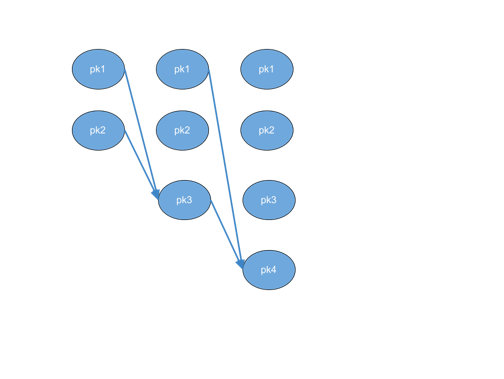
\includegraphics[width=\textwidth]{images/monero/ring_sing_ex.png}
        \caption{}
        \label{fig:f1}
    \end{subfigure}
    \begin{subfigure}[b]{0.5\textwidth}
        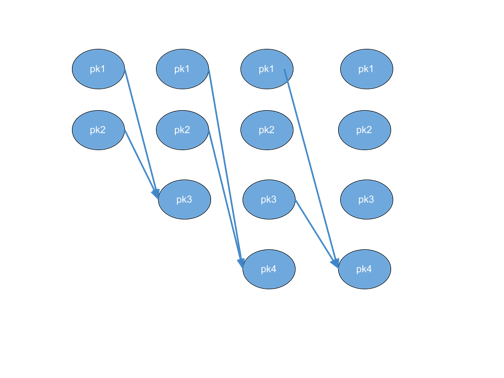
\includegraphics[width=\textwidth]{images/monero/ring_sing__bad_ex.png}
        \caption{}
        \label{fig:f2}
    \end{subfigure}
    \caption{Ring signature example. \autoref{fig:f1} Either one of $\pk_1, \pk_2$ sends to $\pk_3$, so none of them can be removed from utxo. \autoref{fig:f2} There are cases where anonymity is not guaranteed. Both $\pk_1, \pk_2$ is spent after second transaction, so $\pk_3$ is the sender of the third transaction.}
    \label{fig:ring-sig-ex}
\end{figure}

\subsubsection{Stealth addresses}

In order to improve its anonymity, each Monero transaction generates a one-time destination address, known as a stealth address. This address is derived from the recipient's public key, but is unique for each transaction, ensuring that the recipient's public address remains private.

An example of such addresses is presented bellow implemented using elliptic curves:

Let Alice be the sender and Bob the receiver. Bob owns a key-pair of the form $\pk = (A,B), \sk = (a,b)$ such that $A = aG, B= bG$ where $G$ is the base of the used elliptic curve. Then Alice generates a random $r$ and calculates $P = H{rA}G + B$, where $H$ is a collision-resistant hash function. Alice publishes $P, R = rG$ together with the transaction. Afterwards, Bob can check if $P^\prime = H{aR}G + B$. If the transaction is destined for Bob then it holds that $P^\prime = P$.

Obviously, no one will know that this address is intended for Bob, but only Bob can prove that this address is associated with him. In this way, Monero hides the recipient address of the transaction.

% \subsubsection{Ring Confidential Transactions} 